%!TEX root = ../../scivis_lbaakman_bvanloon.tex
\section{Results}
\label{s:streamlines:results}
All images of streamlines computed in this section represent the state of the simulation as visualized by 

\begin{figure}
	\centering
	\begin{subfigure}{0.49\textwidth}
		\centering
		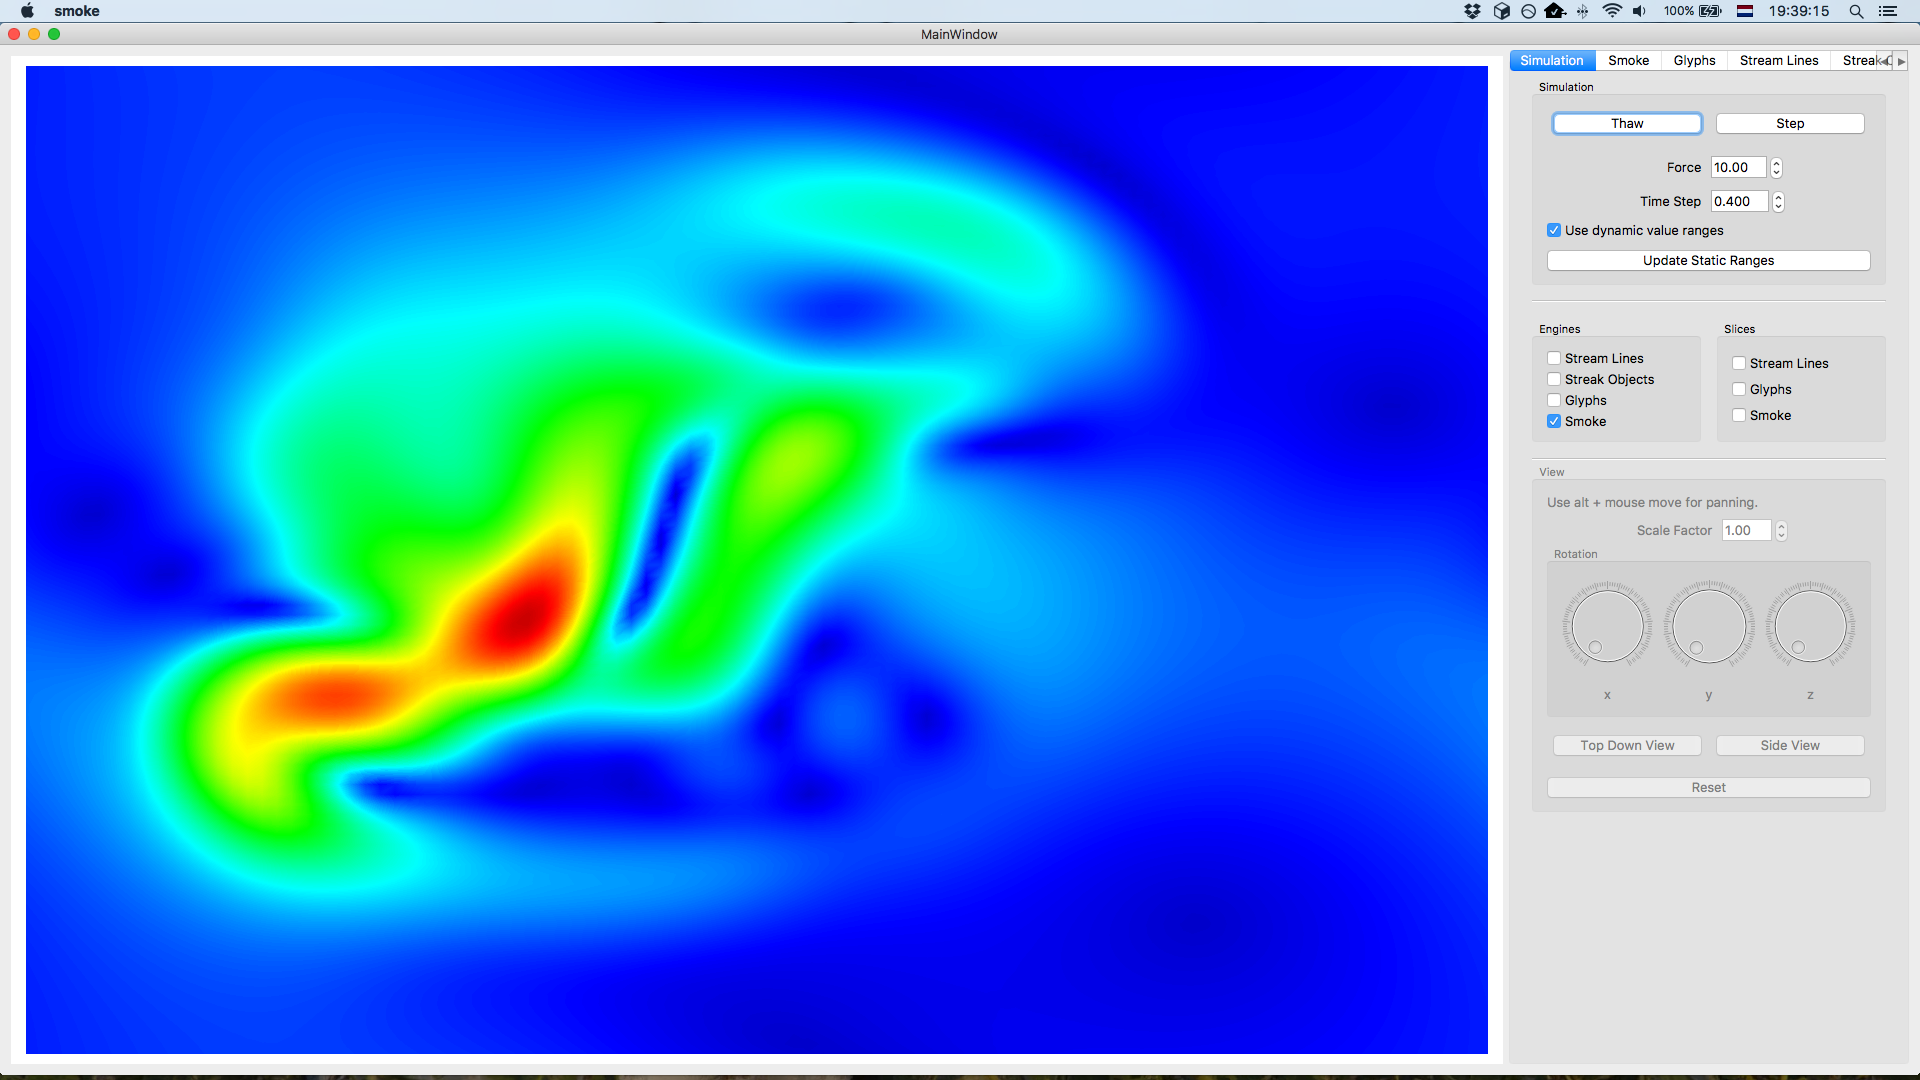
\includegraphics[width=\textwidth]{img/streamlines/simulationStateSmoke.png}
		\caption{\velocitymagnitude}
		\label{fig:streamlines:results:simulationstate:smoke}
	\end{subfigure}
	\begin{subfigure}{0.49\textwidth}
		\centering
		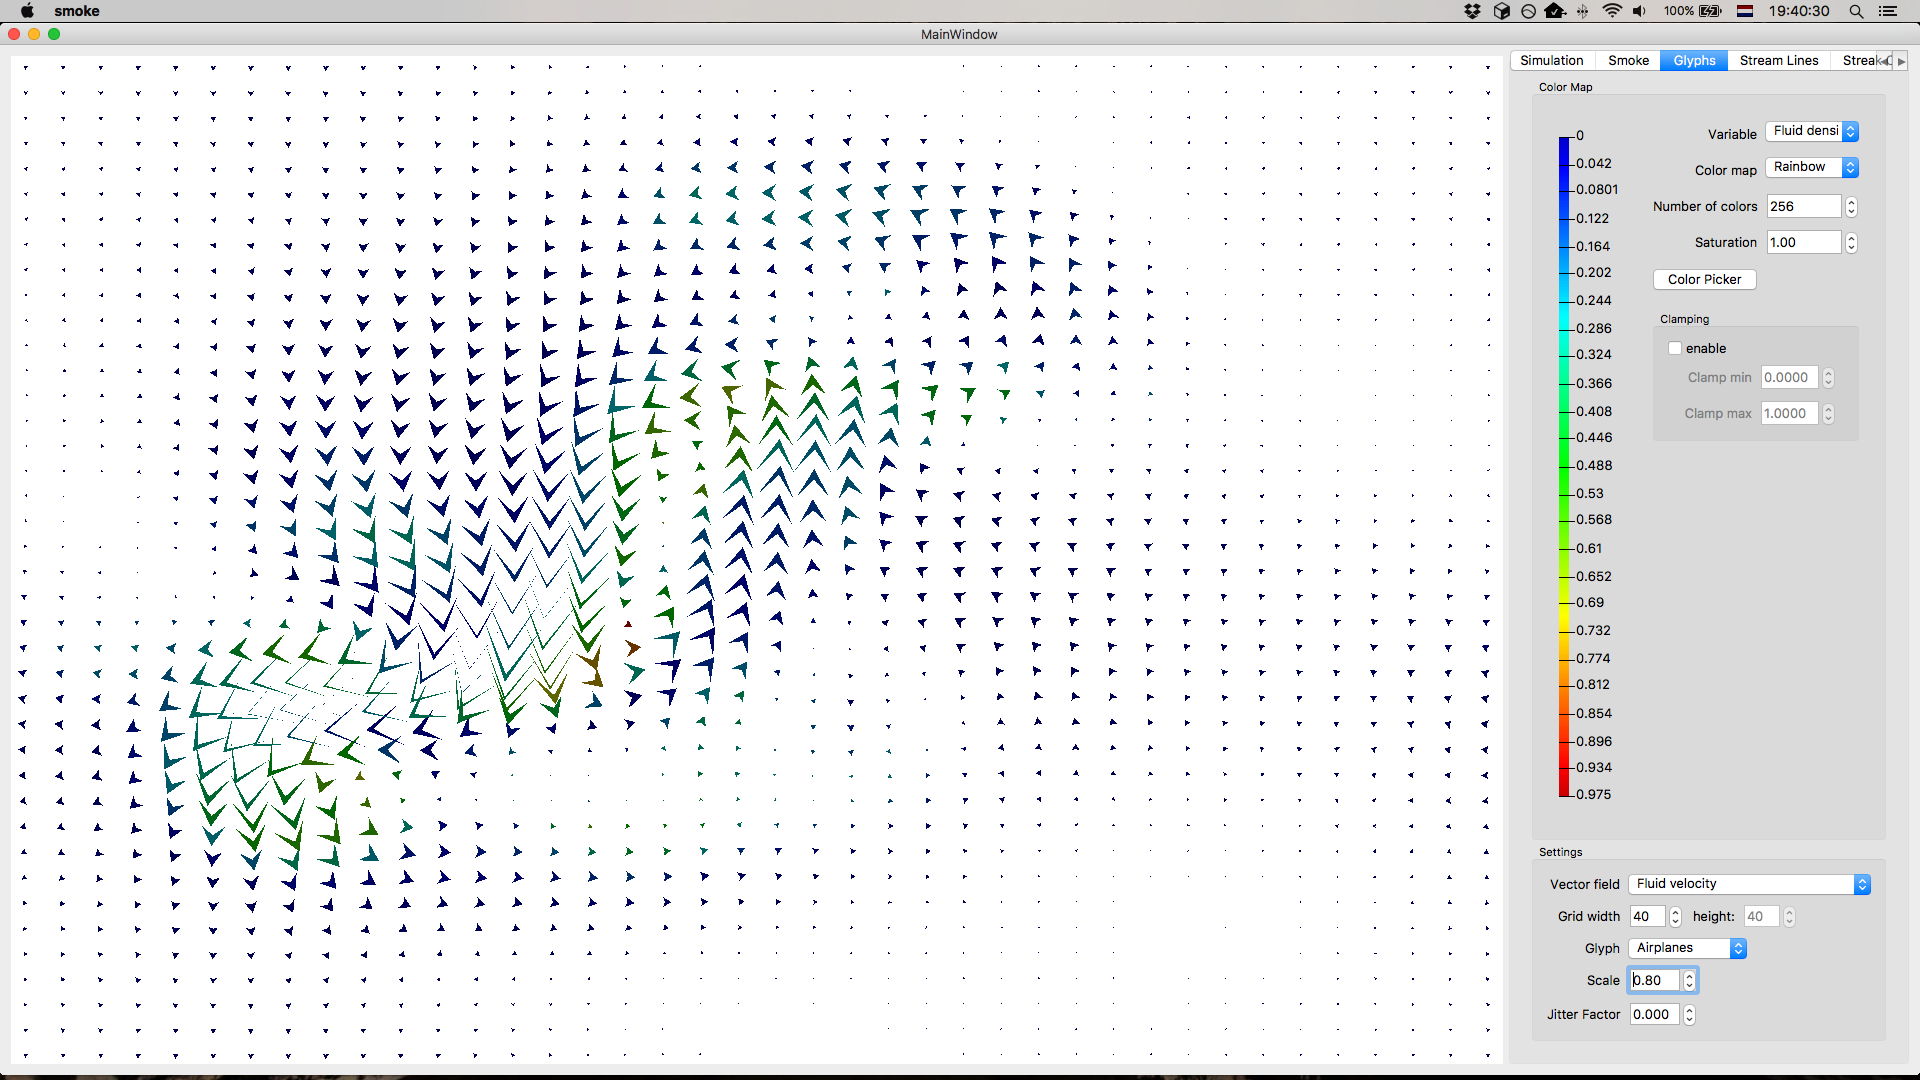
\includegraphics[width=\textwidth]{img/streamlines/simulationStateGlyphs.png}
		\caption{\velocity}
		\label{fig:streamlines:results:simulationstate:glyphs}
	\end{subfigure}	
	\caption{A visualization of the \subref{fig:streamlines:results:simulationstate:smoke} \velocitymagnitude and \subref{fig:streamlines:results:simulationstate:glyphs} \velocity of the vector field used to illustrate the visualization of streamlines in this section.}
	\label{fig:streamlines:results:simulationstate}
\end{figure}


\todo[inline]{Show streamlines when seeded on a few points, show both smoke and streamline visualization}
\todo[inline]{Discuss differences}



\todo[inline]{Show streamlines of state x when seeded on a grid with different minimum magnitudes}
\todo[inline]{Discuss differences}

\todo[inline]{Show streamlines of state x when seeded on a grid with different time steps}
\todo[inline]{Discuss differences}

\todo[inline]{Show streamlines of state x when seeded on a grid with different edge lengths}
\todo[inline]{Discuss differences}

\todo[inline]{Discuss that we didn't move the streamlines until the end of the computational domain}
